\documentclass{article}

% Formatting
\usepackage[utf8]{inputenc}
\usepackage[margin=1in]{geometry}
\usepackage[titletoc,title]{appendix}
\usepackage[spanish]{babel}
\usepackage{amsmath,amsfonts,amssymb,mathtools}
\usepackage{graphicx,float}
\usepackage[ruled,vlined]{algorithm2e}
\usepackage{algorithmic}
\usepackage{minted}
\usemintedstyle{borland}
\usepackage{subcaption}
\usepackage{multicol}
\usepackage{listings}
\usepackage{xcolor}
\usepackage{biblatex}
\addbibresource{ref.bib}
\usepackage{minted}



% Title content
\title{Práctica 11 frentes de Pareto}
\author{Denisse Leyva}
\date{Mayo 12, 2021}

\begin{document}

\maketitle


\section{Introducción}
En optimización multicriterio, a un mismo conjunto de variables ocupa asignarse valores de tal forma que se optimizen dos o más funciones objetivo, que pueden contradecir una a otra, una mejora en una puede corresponder en una empeora en otra. Además hay que respetar potenciales restricciones, si es que haya.

Para estudiar este problema, vamos a primero implementar un generador de polinomios aleatorios. Estos polinomios los utilizaremos como funciones objetivo. Vamos a permitir solamente una variable por término y un término por grado por variable.

Para simplicidad de visualización, vamos a concentrarnos en el caso de dos funciones objetivo. Vamos a generar muchas soluciones al azar, también por simplicidad, los retos de la tarea permitirán mejorar este aspecto, y calculamos los valores de los objetivos para cada solución. Por simplicidad, vamos a suponer que no tenemos restricciones.
Para cada objetivo, vamos a determinar si se va a minimizar (los marcamos con verdad) o maximizar (los marcamos con false). Marcamos con colores distintos las mejores soluciones de cada objetivo.

Como los dos mejores rara vez logran a coincidir y a veces son bastante opuestos, se ocupa una definición para qué en sí es una buena solución. Para eso usaremos la dominancia de Pareto: una solución domina a otra si no empeora ninguno de los objetivos y mejora a por lo menos uno. Vamos a calcular la dominancia en paralelo entre todas las soluciones y marcar aquellas que no son dominadas por ninguna otra solución \cite{Satu_Elisa_Schaeffer}.

\section{Objetivo}
Grafica el porcentaje de soluciones de Pareto (ojo, no es lo mismo que se grafica en el código ejemplo) como función del número de funciones objetivo para $k \in [2, 8]$  en pasos de dos con diagramas de violín combinados con diagramas de caja-bigote, verificando que diferencias observadas, cuando las haya, sean estadísticamente significativas. Razona en escrito a qué se debe el comportamiento observado \cite{Satu_Elisa_Schaeffer}.

\newpage
\section{Código}
El código base se sacó de Schaeffer \cite{Elisa_Schaeffer}. El código completo se encuentra en el GitHub \cite{Denisse_Leyva}.

\renewcommand{\listingscaption}{Código}
\begin{listing}[H]
  \begin{minted}[linenos,mathescape,texcl]{clojure}
iteracion = 100 # cuantas iteraciones
porcentajes = []
for k in range(2, 9, 2): # cuantas funciones objetivo
    for it in range(iteracion): 
        vc = 4
        md = 3
        tc = 5
        obj = [poli(md, vc, tc) for i in range(k)]
        minim = np.random.rand(k) > 0.5
        n = 250 # cuantas soluciones aleatorias
        sol = np.random.rand(n, vc)
        val = np.zeros((n, k))
        for i in range(n): # evaluamos las soluciones
            for j in range(k):
                val[i, j] = evaluate(obj[j], sol[i])
        sign = [1 + -2 * m for m in minim]
        no_dom = []
        for i in range(n):
            d = [domin_by(sign * val[i], sign * val[j]) for j in range(n)]
            no_dom.append(not np.any(d)) # si es cierto que ninguno es verdadero
        frente = val[no_dom, :]
        porcentaje = (len(frente)/n)*100
        porcentajes.append(porcentaje)
      \end{minted}
  \label{lst:fibo}
  \caption{Automatización para obtener las funciones objetivo de la 2 a la 8 de dos en dos.}
\end{listing}

\section{Resultados}
Como se puede observar en la gráfica dependiendo de las funciones objetivo entre menor sean, menor será el porcentaje de Pareto obtenido.
Sin embargo, a más objetivos se puede observar que sube linealmente a cubrir casi el 100 $\%$ con el frente de Pareto. Esto se debe a que al momento de agregar más dimensiones el frente de Pareto por lógica va a ocupar mucho más espacio.

\begin{figure}[H]
\centering
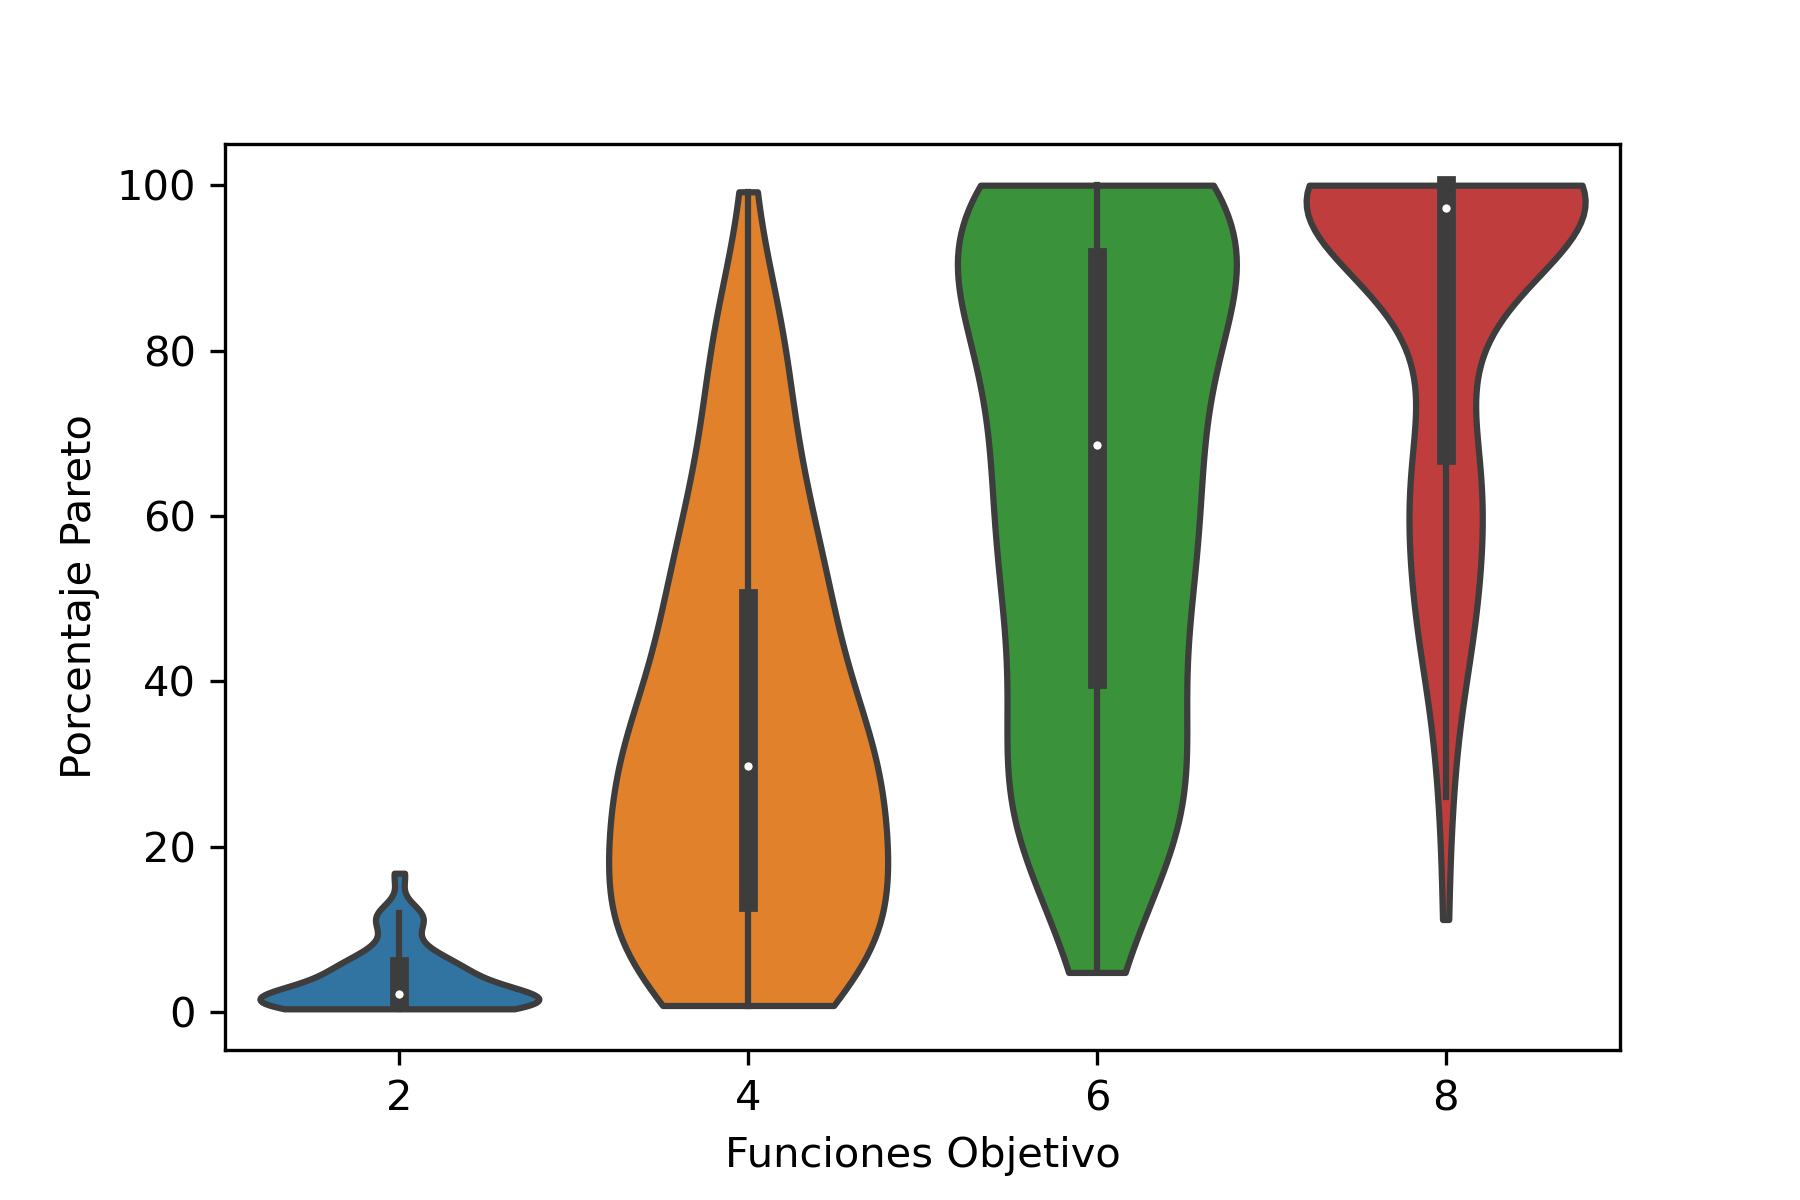
\includegraphics[width=80mm]{p11p.png}
\caption{\label{fig3} Gráfica violín de las funciones objetivo vs porcentaje Pareto.}
\end{figure}

\section{Reto 1}
El primer reto es seleccionar un subconjunto (cuyo tamaño como un porcentaje del frente original se proporciona como un parámetro) del frente de Pareto de tal forma que la selección esté diversificada, es decir, que no estén agrupados juntos en una sola zona del frente las soluciones seleccionadas. Graficar los resultados de la selección, indicando con un color cuáles se incluyen en el subconjunto diverso \cite{Satu_Elisa_Schaeffer}.

\printbibliography

\end{document}
